\documentclass[xcolor=svgnames, 10pt, handout, standalone]{beamer}
\input{beamerUVApreamble}
\usepackage{microtype}
\usepackage{multicol}
\usepackage{bm}
\usepackage{etoolbox}
\usepackage{tcolorbox}
\tcbuselibrary{skins}  % This enables drop shadow and other styling options
\usepackage{tikz}
\usetikzlibrary{shapes, arrows, positioning, calc}

% SHORTCUTS
\newcommand{\Var}{\operatorname{Var}}
\newcommand{\Cov}{\operatorname{Cov}}
\newcommand{\1}{\mathbf{1}}
\newcommand{\R}{\mathbb{R}}
\newcommand{\KL}{\mathrm{D}_{\mathrm{KL}}}
\newcommand{\I}{\mathbf{I}}
\newcommand{\softmax}{\operatorname{softmax}}
\newcommand{\principle}[1]{\textbf{#1}}
\newcommand{\reasonprompt}[1]{\par\small\emph{Reasoning prompt:} #1}
\definecolor{deepblue}{RGB}{0,51,102}
\definecolor{deepgreen}{RGB}{0,102,51}
\definecolor{deepred}{RGB}{153,0,0}
\definecolor{lightblue}{RGB}{230,240,250}
\definecolor{lightyellow}{RGB}{255,250,230}
\definecolor{vibrantblue}{RGB}{0,123,255}
\definecolor{energyorange}{RGB}{255,149,0} 
\definecolor{hotpink}{RGB}{255,45,85}
\definecolor{electricpurple}{RGB}{147,51,234}
\definecolor{neongreen}{RGB}{57,255,20}

% TITLE INFO
\title[Universal Approximation]{Universal Approximation Theory\\and Network Expressivity}
\author{Heman Shakeri}
\date{}

\begin{document}

% Title slide
\begin{frame}
\titlepage
\end{frame}

% Outline
\begin{frame}{Outline}
\tableofcontents
\end{frame}

% Section 1: Introduction
\section{Introduction: The Fundamental Questions}

\begin{frame}{The Fundamental Questions of Neural Networks}
\begin{block}{Can neural networks approximate ANY function?}
\begin{itemize}
    \item What functions can neural networks represent?
    \item Are there theoretical limits?
    \item How does architecture affect expressivity?
\end{itemize}
\end{block}

\begin{alertblock}{Two Landmark Results}
\begin{enumerate}
    \item \textbf{Universal Approximation Theorem}: Shallow networks suffice in theory
    \item \textbf{Depth Efficiency}: Deep networks win in practice
\end{enumerate}
\end{alertblock}
\end{frame}

\begin{frame}{Roadmap for Today}
\begin{enumerate}
    \item<1-> Review: Shallow neural networks as piecewise linear functions
    \item<2-> The Universal Approximation Theorem (UAT)
    \item<3-> Circuit theory and exponential separations
    \item<4-> Deep networks: hierarchical composition
    \item<5-> Practical design principles
\end{enumerate}

\onslide<6->
\begin{center}
\textit{``In theory, theory and practice are the same.\\
In practice, they are not.'' -- Attributed to Yogi Berra}
\end{center}
\end{frame}

% Section 2: Shallow Networks
\section{Shallow Neural Networks: Building Blocks}

\begin{frame}{Shallow Network Architecture}
\begin{columns}
\column{0.5\textwidth}
\textbf{Mathematical Form:}
\begin{equation}
f(x; W, b) = b_0 + \sum_{d=1}^{D} w_d \cdot a[b_d + w_{d,in} \cdot x]
\end{equation}

Where:
\begin{itemize}
    \item $D$ = number of hidden units
    \item $a[\cdot]$ = activation (ReLU)
    \item $W, b$ = weights and biases
\end{itemize}

\column{0.5\textwidth}
\textbf{Key Properties:}
\begin{itemize}
    \item Each hidden unit creates one ``joint''
    \item $D$ units $\rightarrow$ up to $D+1$ linear regions
    \item Piecewise linear output
\end{itemize}
\end{columns}
\end{frame}

\begin{frame}{Visualization: How Shallow Networks Build Functions}
\begin{center}
\includegraphics[width=0.5\textwidth]{Module 1/Fig3.3.png}\\
{\tiny \centering [From Prince, Understanding Deep Learning, Figure 3.3]}
\end{center}

\pause
\textbf{Key insight:} Network ``stitches together'' linear pieces
\end{frame}

\begin{frame}{Increasing Capacity: More Hidden Units}
\begin{center}
\includegraphics[width=0.9\textwidth]{Module 1/Fig3.5.png}\\
{\tiny \centering [From Prince, Understanding Deep Learning, Figure 3.5]}
\end{center}

\pause
As $D \to \infty$: Can approximate \textit{any} continuous function!
\end{frame}

% Section 3: Universal Approximation
\section{The Universal Approximation Theorem}

\begin{frame}{Universal Approximation Theorem (UAT)}
\begin{theorem}[Universal Approximation - Cybenko 1989, Hornik 1991]
For any continuous function $f: K \subset \mathbb{R}^n \to \mathbb{R}^m$ on compact $K$, and any $\epsilon > 0$:

\textbf{There exists} a shallow neural network $g$ with finite hidden units such that:
\begin{equation}
\sup_{x \in K} ||f(x) - g(x)|| < \epsilon
\end{equation}
\end{theorem}

\pause
\begin{center}
\Large{\textbf{Translation: Shallow networks can approximate\\ANY continuous function!}}
\end{center}
\end{frame}

\begin{frame}{The Intuition Behind UAT}
\begin{columns}
\column{0.5\textwidth}
\textbf{The Recipe:}
\begin{enumerate}
    \item<1-> Add more hidden units
    \item<2-> Get more linear regions
    \item<3-> Regions become smaller
    \item<4-> Better local approximation
    \item<5-> Arbitrarily good fit!
\end{enumerate}

\column{0.5\textwidth}
\onslide<6->
\textbf{Think of it as:}
\begin{itemize}
    \item Approximating curves with many tiny line segments
    \item Like pixels approximating an image
    \item Resolution $\uparrow$ as neurons $\uparrow$
\end{itemize}
\end{columns}
\end{frame}

\begin{frame}{What UAT Guarantees (and What It Doesn't)}

\textbf{The theorem guarantees:}
\begin{itemize}
    \item[\checkmark] A network \textit{exists} that can approximate any continuous function
\end{itemize}

\textbf{The theorem does NOT tell us:}
\begin{itemize}
    \item[$\times$] How to find the weights (training algorithm)
    \item[$\times$] How many neurons we need (could be exponentially many!)
    \item[$\times$] Whether we can train it efficiently
\end{itemize}

\begin{alertblock}{Critical Point}
UAT says a network \textit{exists}, but doesn't tell us how to find it or how big it needs to be!
\end{alertblock}
\end{frame}

% Section 4: Circuit Theory
\section{Circuit Theory and Exponential Separations}

% \begin{frame}{Circuit Theory and Deep Learning}
% \begin{block}{Core Result (Informal)}
% There are functions you can compute with a ``small'' $L$-layer deep neural network that shallower networks require exponentially more hidden units to compute.
% \end{block}

% \pause
% % \begin{center}
% \includegraphics[width=0.7\textwidth]{circuit_theory_xor.png}
% \end{center}

% \pause
% \textbf{Key Example:} $n$-way XOR = $x_1 \oplus x_2 \oplus \ldots \oplus x_n$
% \end{frame}

\begin{frame}{The XOR Example: Exponential Separation}
\textbf{Computing parity of $n$ bits:} $y = x_1 \oplus x_2 \oplus \ldots \oplus x_n$

\vspace{0.5em}
\begin{columns}[T]
\column{0.48\textwidth}
\begin{block}{Deep Network Solution}
\begin{itemize}
    \item Build a tree of XOR operations
    \item Hierarchical computation
    \item \textbf{Depth:} $O(\log n)$
    \item \textbf{Total neurons:} $O(n)$
\end{itemize}
\end{block}

\column{0.48\textwidth}
\begin{block}{Shallow Network Problem}
\begin{itemize}
    \item Must ``memorize'' all combinations
    \item No hierarchical reuse
    \item \textbf{Depth:} 1
    \item \textbf{Hidden neurons:} $\sim 2^n$
\end{itemize}
\end{block}
\end{columns}

\pause
\vspace{0.5em}
\begin{alertblock}{Exponential Gap!}
Deep: $O(n)$ neurons vs Shallow: $O(2^n)$ neurons
\end{alertblock}
\end{frame}

\begin{frame}{Intuition: Why Depth Provides Exponential Advantage}
\begin{center}
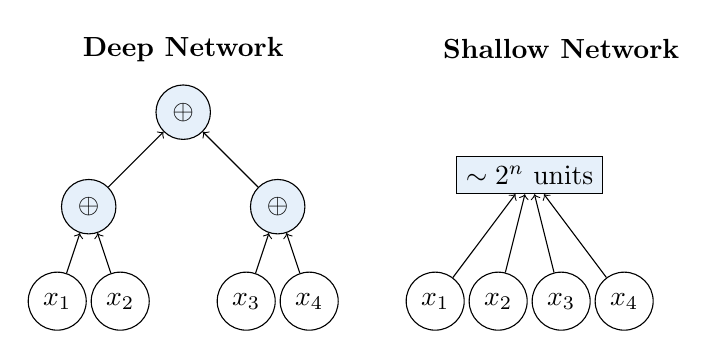
\begin{tikzpicture}[scale=0.8]
    % Deep network (tree structure)
    \node at (-3, 4) {\textbf{Deep Network}};
    \node[circle, draw] (x1) at (-5, 0) {$x_1$};
    \node[circle, draw] (x2) at (-4, 0) {$x_2$};
    \node[circle, draw] (x3) at (-2, 0) {$x_3$};
    \node[circle, draw] (x4) at (-1, 0) {$x_4$};
    
    \node[circle, draw, fill=lightblue] (h11) at (-4.5, 1.5) {$\oplus$};
    \node[circle, draw, fill=lightblue] (h12) at (-1.5, 1.5) {$\oplus$};
    
    \node[circle, draw, fill=lightblue] (h21) at (-3, 3) {$\oplus$};
    
    \draw[->] (x1) -- (h11);
    \draw[->] (x2) -- (h11);
    \draw[->] (x3) -- (h12);
    \draw[->] (x4) -- (h12);
    \draw[->] (h11) -- (h21);
    \draw[->] (h12) -- (h21);
    
    % Shallow network (all-to-all)
    \node at (3, 4) {\textbf{Shallow Network}};
    \node[circle, draw] (sx1) at (1, 0) {$x_1$};
    \node[circle, draw] (sx2) at (2, 0) {$x_2$};
    \node[circle, draw] (sx3) at (3, 0) {$x_3$};
    \node[circle, draw] (sx4) at (4, 0) {$x_4$};
    
    \node[rectangle, draw, fill=lightblue] (sh1) at (2.5, 2) {$\sim 2^n$ units};
    
    \draw[->] (sx1) -- (sh1);
    \draw[->] (sx2) -- (sh1);
    \draw[->] (sx3) -- (sh1);
    \draw[->] (sx4) -- (sh1);
\end{tikzpicture}
\end{center}

\textbf{Deep:} Hierarchical reuse of computations\\
\textbf{Shallow:} Must enumerate all possible cases
\end{frame}

% Section 5: Deep Networks
\section{Deep Networks and Hierarchical Composition}

\begin{frame}{Linear Regions: Shallow vs Deep}
\begin{columns}
\column{0.5\textwidth}
\textbf{Shallow Network (1 layer):}
\begin{itemize}
    \item Parameters: $\sim 3D$
    \item Max regions: $D + 1$
    \item Growth: \textcolor{red}{Linear}
\end{itemize}

\vspace{0.5cm}

\textbf{Deep Network ($K$ layers):}
\begin{itemize}
    \item Parameters: $\sim KD^2$
    \item Max regions: $(D+1)^K$
    \item Growth: \textcolor{green}{Exponential!}
\end{itemize}

\column{0.5\textwidth}
\onslide<2->
\textbf{Example with $D=10$:}
\begin{itemize}
    \item 1 layer: 11 regions
    \item 2 layers: 121 regions
    \item 3 layers: 1,331 regions
    \item 5 layers: \textbf{161,051 regions!}
\end{itemize}
\end{columns}
\end{frame}

\begin{frame}{Two Views of Deep Networks}
\begin{block}{View 1: Folding Space}
Deep networks progressively ``fold'' the input space:
\begin{itemize}
    \item Layer 1: Simple linear boundaries
    \item Layer 2: Combines boundaries $\rightarrow$ complex regions
    \item Layer 3+: Increasingly intricate decision boundaries
\end{itemize}
\end{block}

\pause

\begin{block}{View 2: Hierarchical Feature Learning}
\begin{center}
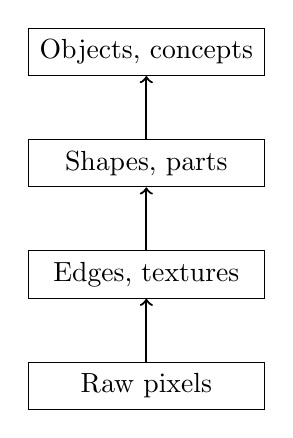
\begin{tikzpicture}[
    layer/.style={rectangle, draw, minimum width=3cm, minimum height=0.6cm, align=center},
    arrow/.style={->, thick}
]
    \node[layer] (input) {Raw pixels};
    \node[layer, above=0.8cm of input] (layer1) {Edges, textures};
    \node[layer, above=0.8cm of layer1] (layer2) {Shapes, parts};
    \node[layer, above=0.8cm of layer2] (output) {Objects, concepts};
    
    \draw[arrow] (input) -- (layer1);
    \draw[arrow] (layer1) -- (layer2);
    \draw[arrow] (layer2) -- (output);
\end{tikzpicture}
\end{center}
\end{block}
\end{frame}

\begin{frame}{Empirical Evidence: Regions vs Parameters}
\begin{center}
\includegraphics[width=0.5\textwidth]{Module 1/Fig4.7a.png}
\end{center}
{\footnotesize \centering From Prince, Understanding Deep Learning, Figure 4.7a}

\pause
\textbf{Key observation:} For fixed parameter budget, deeper is exponentially better!
\end{frame}

\begin{frame}{Theoretical Foundation: Liang \& Srikant (2017)}
\begin{center}
\includegraphics[width=0.4\textwidth]{Module 1/LiangSrikantpaper.png}
\end{center}

\pause
\begin{block}{Main Result}
For piecewise smooth functions with approximation error $\epsilon$:
\begin{itemize}
    \item Shallow networks need: $\Omega(\text{poly}(1/\epsilon))$ neurons
    \item Deep networks need: $O(\text{polylog}(1/\epsilon))$ neurons
\end{itemize}
\textbf{Exponential difference in efficiency!}
\end{block}
\end{frame}

% Section 6: Design Principles
\section{Practical Design Principles}

\begin{frame}{The Expressivity-Trainability-Efficiency Triangle}
\begin{center}
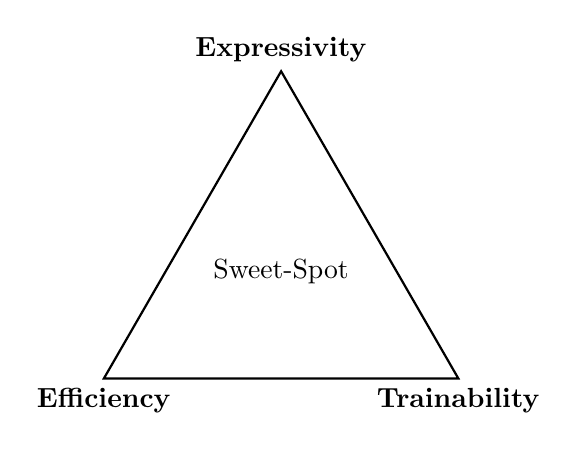
\begin{tikzpicture}[scale=1.5]
    \coordinate (A) at (0,0);
    \coordinate (B) at (3,0);
    \coordinate (C) at (1.5,2.6);
    
    \draw[thick] (A) -- (B) -- (C) -- cycle;
    
    \node[below] at (A) {\textbf{Efficiency}};
    \node[below] at (B) {\textbf{Trainability}};
    \node[above] at (C) {\textbf{Expressivity}};
    
    \node at (1.5,0.9) {Sweet-Spot};
    
    % \pause
    % % Examples
    % \node[text=deepgreen] at (-0.5,1.5) {ResNet};
    % \draw[->, deepgreen] (-0.2,1.4) -- (1.2,1.2);
    
    % \node[text=deepblue] at (3.5,1.5) {Attention};
    % \draw[->, deepblue] (3.2,1.4) -- (1.8,1.2);
\end{tikzpicture}
\end{center}

\pause
\textbf{Good designs improve at least two corners:}
\begin{itemize}
    \item ResNet: Better trainability AND expressivity
    \item Attention: Better expressivity AND efficiency
\end{itemize}
\end{frame}

\begin{frame}{Core Design Principles}
\begin{overlayarea}{\textwidth}{0.7\textheight}
\only<1>{
\begin{block}{Principle 1: Maximize Useful Nonlinearity per Parameter}
\begin{itemize}
    \item Exponential growth of regions with depth
    \item Prefer designs that buy many decision regions per parameter
    \item Balance: modest width, adequate depth, parameter reuse
    \item ``Useful'' = what optimization can reliably access
\end{itemize}
\end{block}}

\only<2>{
\begin{block}{Principle 2: Depth is Leverage, Width is Comfort}
\begin{itemize}
    \item Adding layers: Multiplies representational power
    \item Adding width: Linear capacity increase, diminishing returns
    \item Deep networks exploit hierarchical composition
    \item Width helps optimization but doesn't fundamentally change expressivity
\end{itemize}
\end{block}}

\only<3>{
\begin{block}{Principle 3: Expressivity is Cheap, Trainability is the Gatekeeper}
\begin{itemize}
    \item UAT guarantees existence, not learnability
    \item Initialization, normalization, residual connections matter
    \item Choose deepest model you can \emph{stably} optimize
    \item Monitor gradient flow and adjust accordingly
\end{itemize}
\end{block}}

\only<4>{
\begin{block}{Principle 4: Use Structure to Buy More Function per Parameter}
\begin{itemize}
    \item Convolution: Spatial parameter sharing
    \item Recurrence: Temporal parameter sharing  
    \item Attention: Dynamic, content-based computation
    \item Sparse/conditional compute: Activate only relevant paths
\end{itemize}
\end{block}}
\end{overlayarea}
\end{frame}

\begin{frame}{Design Checklist for Any New Layer/Block}
\begin{enumerate}
    \item<2-> Does it add \emph{useful} nonlinearity per parameter/FLOP?
    \item<3-> Does it prefer depth/composition over naive width?
    \item<4-> Is it trainable with our init/norm/optimizer?
    \item<5-> Does it exploit structure/weight sharing?
    \item<6-> Does it enable conditional/sparse compute?
    \item<7-> Does it improve margins and stay calibrated?
    \item<8-> Do our metrics capture its trade-offs?
    \item<9-> Does it move at least two corners of the Triangle?
\end{enumerate}
\end{frame}



\section{Practical Implications}

\begin{frame}{When to Use Shallow vs Deep}
\begin{columns}
\column{0.5\textwidth}
\textbf{Use Shallow Networks for:}
\begin{itemize}
    \item Simple, smooth functions
    \item Limited training data
    \item Interpretability critical
    \item Real-time inference
    \item Theoretical guarantees needed
\end{itemize}

\column{0.5\textwidth}
\textbf{Use Deep Networks for:}
\begin{itemize}
    \item Complex patterns (images, text)
    \item Hierarchical structure
    \item Abundant training data
    \item Parameter efficiency matters
    \item State-of-the-art performance
\end{itemize}
\end{columns}

\pause
\vspace{0.5cm}
\begin{center}
\textbf{Modern reality: Deep almost always wins in practice!}
\end{center}
\end{frame}

\begin{frame}{Concrete Example: Function Approximation}
\textbf{Task: Approximate $f(x) = \sin(10x)$ on $[0, 2\pi]$ with error $< 0.01$}

\vspace{0.5cm}

\begin{columns}
\column{0.5\textwidth}
\textbf{Shallow Approach:}
\begin{itemize}
    \item Need to capture all oscillations
    \item Each neuron = 1 linear piece
    \item Required: $\sim$100 neurons
    \item Parameters: $\sim$300
\end{itemize}

\column{0.5\textwidth}
\textbf{Deep Approach:}
\begin{itemize}
    \item Layer 1: Learn frequency
    \item Layer 2: Combine patterns
    \item Required: $\sim$20 total neurons
    \item Parameters: $\sim$150
\end{itemize}
\end{columns}

\pause
\centering
50\% parameter reduction through depth!
\end{frame}

% Section 8: Summary
\section{Summary and Key Takeaways}

\begin{frame}{The Big Picture}
\begin{center}
\Large{\textbf{Universal Approximation tells us\\what's POSSIBLE}}

\vspace{0.5cm}

\Large{\textbf{Circuit Theory tells us\\what's EFFICIENT}}

\vspace{0.5cm}

\Large{\textbf{Deep Learning shows us\\what's PRACTICAL}}
\end{center}
\end{frame}

\begin{frame}{Key Takeaways}
\begin{enumerate}
    \item<1-> \textbf{Universal Approximation:} Shallow networks CAN approximate any continuous function
    \vspace{0.3cm}
    \item<2-> \textbf{The Catch:} May need exponentially many neurons!
    \vspace{0.3cm}
    \item<3-> \textbf{Circuit Theory:} Some functions have exponential separations between shallow and deep (cost in terms of number of neurons or logic gates)
    \vspace{0.3cm}
    \item<4-> \textbf{Depth Efficiency:} Deep networks are exponentially more parameter-efficient
    \vspace{0.3cm}
    \item<5-> \textbf{Design Principle:} Maximize the expressivity-trainability-efficiency triangle
\end{enumerate}
\end{frame}

\begin{frame}{Remember This}
\begin{block}{The Success of Deep Learning}
Deep learning succeeds because of:
\begin{itemize}
    \item Theoretical expressivity (UAT + Circuit Theory)
    \item Practical efficiency (depth advantage)
    \item Hierarchical inductive biases
    \item Better optimization algorithms
    \item More data and compute
\end{itemize}
\end{block}

\pause
\vspace{0.5cm}
\begin{center}
\textit{``With four parameters I can fit an elephant,\\
and with five I can make him wiggle his trunk.''}\\
-- John von Neumann

\vspace{0.3cm}
\textbf{But with depth, we can do it efficiently!}
\end{center}
\end{frame}

\begin{frame}{Looking Ahead}
\textbf{Next Topics:}
\begin{itemize}
    \item How do we actually FIND these good approximations? (Optimization)
    \item Why do deep networks generalize well? (Learning theory)
    \item What architectures work best? (CNNs, Transformers)
\end{itemize}

\vspace{0.5cm}

\textbf{Reading:}
\begin{itemize}
    \item Prince, Understanding Deep Learning, Chapters 3-4
    \item Original UAT papers: Cybenko (1989), Hornik (1991)
    \item Circuit theory: Håstad (1987), Razborov (1987)
    \item Depth efficiency: Telgarsky (2016), Liang \& Srikant (2017)
\end{itemize}
\end{frame}

\begin{frame}
\begin{center}
\Huge{\textbf{Questions?}}

\vspace{1cm}

\Large{Thank you!}
\end{center}
\end{frame}

\end{document}